
\documentclass[12pt]{article}
\usepackage[a4paper, margin=.30in]{geometry}
\usepackage{graphicx ,
            wrapfig,
            xcolor, 
            enumerate,
            amsmath,
			fontenc,
			tcolorbox
            }

\newcommand\headerMe[2]{\noindent{}#1\hfill#2}
\renewcommand{\thesection}{\Roman{section}}

\author{Zakaria HAOUZAN}
\date{\today}

\begin{document}
% headers --------------
\headerMe{Matière : Physique-Chimie}{Professeur : Zakaria HAOUZAN}\\
\headerMe{Unité : Transformations nucléaires }{Établissement : Lycée SKHOR qualifiant}\\
\headerMe{Niveau : 2BAC-SM-X}{Heure : 4H}\\

% ------Content ________
\begin{center}

    \Large{Leçon $N^{\circ} 4 $: \color{red}Décroissance radioactive. }
\end{center}

%\begin{wrapfigure}[10]{r}{0.5\textwidth}
%    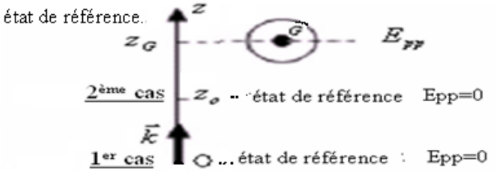
\includegraphics[width=0.5\textwidth]{./img/img00.png}
%\end{wrapfigure}


\section{ Le noyau atomique : }

\subsection{Composition du noyau atomique : }
\begin{itemize}
	\item Le noyau atomique est composé de protons et de neutrons, ces constituants du noyau s'appellent les nucléons.

	\item Le proton a une charge positive appelée charge élémentaire: $q_p=+e=+1,6.10^{-19}C$., 

		sa masse:$m_p$=$1,6726.10^{-27}kg$.
	\item Le neutron est électriquement neutre . $(q_n=0)$. ,sa masse : $m_n=1,6750.10^{ -27}kg$.
\end{itemize}

\subsection{ Représentation symbolique du noyau atomique : }
Le noyau atomique d'un élément chimique est représenté par le symbole: $_Z^AX$

X : symbole de l'élément chimique. \hspace{0.5cm} A: nombre de masse.=nombre de nucléons)

Z: numéro atomique (nombre de protons)  N=A-Z: nombre de neutrons.

Exemple : Donner la composition du noyau dans chacun des cas suivants: $_{92}^{238}U$     $_{11}^{24}Na$ $_{17}^{35}Cl$.

\subsection{Le nucléide : }

Le nucléide étant une espèce atomique, il est défini par le numéro atomique (Z) et par le nombre de masse (A).
Exemple : $_4^2He$ et $_{35}^{17}Cl$ $_{37}^{17}Cl$ - $_{6}^{14}C$ - $_{6}^{13}C$ - $_{6}^{12}C$
\subsection{Les isotopes d’un élément chimique : }

Les isotopes sont les nucléides d'un même élément chimique qui ont le même numéro atomique Z mais
ils diffèrent par leur nombre de masse A : ( ils n'ont pas le même nombre de neutrons). 

Exemples : 
\begin{center}
   \begin{tabular}{ |c|c|c|c| }
	  \hline
	  l'isotope & $_{8}^{16}O$ & $_{8}^{17}O$ & $_{8}^{18}O$ \\\hline
	  \% Abondance & 99,759 & 0,037 & 0,204\\\hline
  \end{tabular}\end{center}


  \section{Stabilité et instabilité des noyaux atomiques: }
  \subsection{La découverte de la radioactivité:}


  \begin{wrapfigure}[7]{r}{0.2\textwidth}
	\vspace{-2cm}
	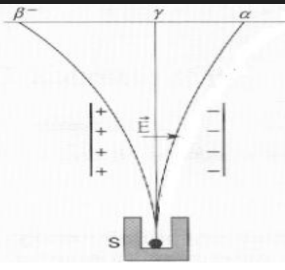
\includegraphics[width=0.2\textwidth]{./img/nuc01.png}
	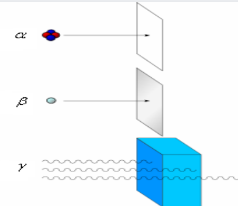
\includegraphics[width=0.2\textwidth]{./img/nuc02.png}
\end{wrapfigure}



La radioactivité naturelle a été découverte par Becquerel en 1896, il remarqua qu'une plaque photographique mise au
voisinage de sels d'uranium avait été impressionnée sans avoir été exposée à la lumière du soleil .

Il en conclut que l'uranium
émet des rayonnements invisibles capables d'impressionner la plaque photographique.

Ensuite on a pu identifier les types rayonnements naturels émis par la matière radioactive à l'aide champ électrique:

Il existe trois types de rayonnements naturels issus de la matière radioactive: les rayons $\alpha$ , les rayons $\beta^-$
et les rayons $\gamma$.

\begin{itemize}
	\item \textbf{Les rayons alpha : }sont des particules matérielles de charges positives, ce sont des noyaux d'hélium, ils peuvent être arrêtés par une feuille de papier .Chaque particule alpha porte une charge positive: $q=+2e$=$2.1,6.10^{-19}C$

	\item \textbf{Les rayons bêta  moins:} sont des électrons, ils sont plus pénétrants que les rayons alpha ,on a besoin d'une plaque
d'aluminium de quelques millimètres ou de verre pour les arrêter.

\item \textbf{ les rayons gamma }: sont des ondes électromagnétiques très énergétiques, ils ont la vitesse de lumière et une grande
capacité de pénétration, pour les arrêter on a besoin d'un mur de béton ou de plomb.
\end{itemize}


\subsection{Définition de la radioactivité : }

La radioactivité est la transformation spontanée d’un noyau atomique instable en un autre plus stable avec émission d'un
rayonnement.,cette transformation s'appelle: "La désintégration radioactive"

\subsection{diagramme de Segré : }
Le diagramme de Segré contient tous les noyaux stables et les noyaux radioactifs existants répartis de la façon suivante: le
nombre de neutrons en abscisse et le nombre de protons en ordonnée: c'est le diagramme (N, Z) 

\begin{center}

	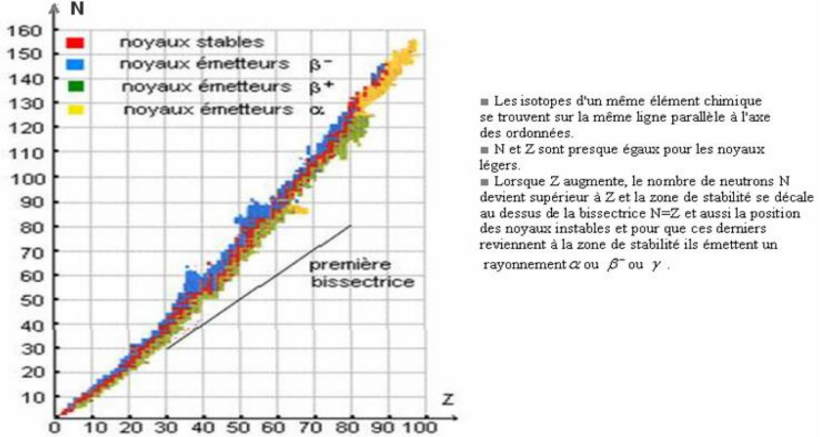
\includegraphics[width=1\textwidth]{./img/nuc03.png}

\end{center}

\section{Transformation Nucléaire Spontanée : }
\subsection{la loi de Conservation de Soddy}
Lors d’une transformation nucléaire, le nombre de nucléons: A et la charge électrique: Z, se conservent.

Appliquons la loi de Soddy à l'équation générale de désintégration suivante: 

$$_Z^AX \rightarrow _{z_1}^{A_1}Y + _{z_2}^{A_2}p$$

\begin{itemize}
	\item X : le noyau père \hspace{0.5cm} Y : le noyau fils \hspace{0.5cm } p : la particule émise pare la désintégration.
	\item Conservation des nucléons : $A = A_2 + A_1$
	\item Conservation du nombre de charge: $Z = Z_1 + Z_2$
\end{itemize}

\subsection{Les différents types de radioactivités : }
\subsubsection{ Radioactivité $\alpha$: }
La radioactivité $\alpha$ est une désintégration nucléaire naturelle, spontanée au cours de laquelle un noyau père $_z^AX$ instable se transforme en un noyau fils $_{z-2}^{A-4}Y$
plus stable avec émission d'une particule $\alpha$.

Remarque: La radioactivité $\alpha$ ne concerne que les noyaux lourds dont le nombre de masse: $A \geq 200$

Equation de désintégration $\alpha$ : $_Z^AX \rightarrow _{Z- 2 }^{A - 4}Y + _{2}^{4}He$

  \begin{wrapfigure}{r}{0.2\textwidth}
	\vspace{-3cm}
	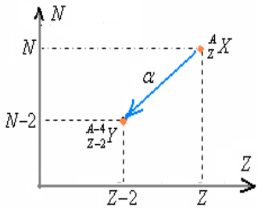
\includegraphics[width=0.2\textwidth]{./img/nuc04.png}
\end{wrapfigure}



\begin{itemize}
	\item désintégration de l'uranium 238 au thorium 234 : $_{92}^{238}U \rightarrow       _{90}^{234}Y + _{2}^{4}He$

	\item désintégration du radium 226 au radon 22 : $_{88}^{226}Ra \rightarrow            _{86}^{222}Rn + _{2}^{4}He$
\end{itemize}

Regardons comment se déplace un nucléide dans le diagramme de Segré après l'émissions d'une particule alpha:

\subsubsection{ Radioactivité $\beta^-$: }

  \begin{wrapfigure}{r}{0.2\textwidth}
	%\vspace{-3cm}
	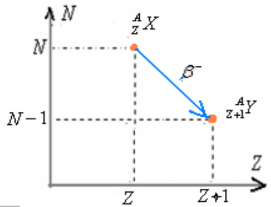
\includegraphics[width=0.2\textwidth]{./img/nuc05.png}
\end{wrapfigure}


La radioactivité $\beta^-$ est une désintégration nucléaire naturelle, spontanée au cours de laquelle un noyau père  $_{z}^{A}X$ instable se transforme en un noyau fils            $_{z+1}^{A}Y$ plus stable avec émission d'un électron $_{-1}^{0}e$ appelé particule $\beta^-$

Equation de désintégration $\beta^-$ : $_Z^AX \rightarrow _{Z+1 }^{A}Y + _{-1}^{0}e$


\begin{itemize}
	\item le Cobalt $_{27}^{60}Co$ il se transforme en nickel, : $_{27}^{60}Co \rightarrow _{28}^{60}Co + _{-1}^{0}e$
	\item Mécanisme : La radioactivité bêta-moins est due à la transformation d'un neutron en un proton dans le noyau: $_0^1n \rightarrow _1^1p + _{-1}^0e$


\end{itemize}
Regardons comment se déplace un nucléide dans le diagramme de Segré après l'émissions d'une particule $\beta^-$



\subsubsection{ Radioactivité $\beta^ +$: }

  \begin{wrapfigure}{r}{0.2\textwidth}
	%\vspace{-3cm}
	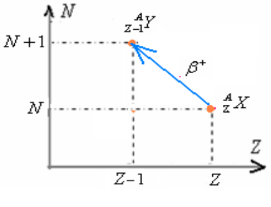
\includegraphics[width=0.2\textwidth]{./img/nuc06.png}
\end{wrapfigure}


La radioactivité $\beta^+$ est une désintégration nucléaire naturelle, spontanée au cours de laquelle un noyau père  $_{Z}^{A}X$ instable se transforme en un noyau fils            $_{X-1}^{A}Y$ plus stable avec émission d'un positron $_{+1}^{0}e$ appelé particule $\beta^+$

Equation de désintégration $\beta^+$ : $_Z^AX \rightarrow _{Z-1 }^{A}Y + _{+1}^{0}e$


\begin{itemize}
	\item désintégration du phosphore en silicium :$_{15}^{30}P \rightarrow _{14}^{30}Si + _{+1}^0e$
	\item Mécanisme : La radioactivité bêta-plus est due à la transformation d'un proton en neutron dans le noyau: $_1^1p \rightarrow _0^1n + _{+1}^0e$


\end{itemize}
Regardons comment se déplace un nucléide dans le diagramme de Segré après l'émissions d'une particule $\beta^+$

\subsubsection{ Radioactivité $\gamma$: }
La désintégration gamma est une désintégration nucléaire naturelle, spontanée qui accompagne les radioactivités $\beta^+$, $\beta^-$, $\alpha$.

En effet , lors des désintégrations $\beta^+$ ou  $\beta^-$, $\alpha$ si le noyau fils est à l'état excité on le note : $_{Z'}^{A'}Y^*$,ce noyau instable perd son excitation en émettant un rayonnement gamma pour se transformer en un noyau $_{Z'}^{A'}Y$ plus stable.



Equation de désintégration $\gamma$ : $_{Z'}^{A'}Y^* \rightarrow _{Z'}^{A'}Y + \gamma$

\begin{itemize}
	\item $_7^{16}N \rightarrow _8^{16}O^* + _{-1}^0e$ c'est une désintégration $\beta^-$ mais le noyau fils n'est pas stable. 
\item $_8^{16}O^* \rightarrow _8^{16}O + \gamma$  il perd son excitation en émettant le rayonnement $\gamma$
\end{itemize}

\subsection{La famille radioactive}
Une famille radioactive est une suite de nucléides descendant d'un même noyau père par une suite de désintégrations successives
jusqu'à l'obtention d'un noyau stable

Exemple : la famille radioactive de l'uranium $_{92}^{238}U$
\begin{center}

	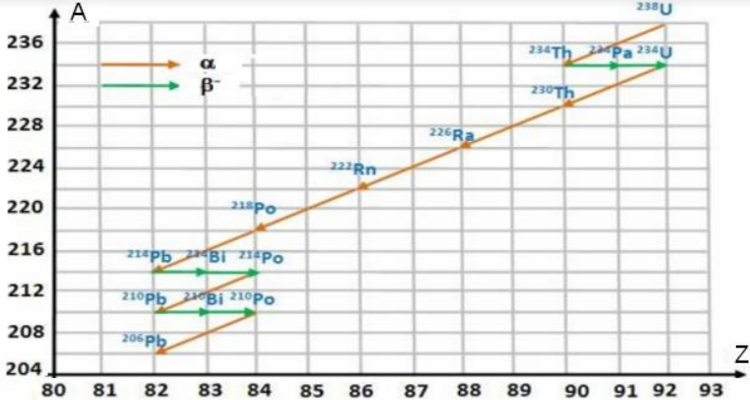
\includegraphics[width=0.8\textwidth]{./img/nuc07.png}
\end{center}
\section{Décroissance radioactive : }
\subsection{Loi de décroissance radioactive:}
La radioactivité est un phénomène spontané aléatoire, on ne peut pas prévoir l'instant de la disintegration et le nombre de
noyaux non désintégrés d'un échantillon radioactif suit la loi de décroissance radioactive suivante: $$N(t) = N_0.e^{-\lambda.t}$$

\begin{itemize}
	\item N(t) : Nombre de noyaux de l'échantillon radioactif restants à l'instant t (non désintégrés). 

	\item $N_0$ Nombre initial de noyaux de l'échantillon radioactif. 

	\item $\lambda$  Constante radioactive, son unité dans le SI est: $s^{-1}$.
	\item Remarque : La constante de temps $\tau = \frac{1}{\lambda}$ est un temps qui caractérise la substance radioactive.
\end{itemize}

\subsection{Demi-vie d'une substance radioactive : }
La demi-vie d'une substance radioactive est le temps mis pour perdre la moitié des noyaux $N_0$ de cette substance initialement présents (à la date t=0).

\begin{itemize}
	\item D'après la loi de décroissance radioactive, le nombre de noyaux restants à l'instant : $N(t) = N_0.e^{-\lambda.t}$. (1)

	\item le nombre de noyaux à $t=t_{1/2}$ :$n(t_{1/2})=\frac{N_0}{2}$ en remplaçant dans (1) $$\frac{N_0}{2} = N_0.e^{-\lambda.t_{1/2}}$$ donc$$t_{1/2} = \frac{ln2}{\lambda}$$
		
		demi-vie d'une substance radioactive

	\item 	Remarque : On peut exprimer la demi-vie en fonction de la constante de temps. 
		$\tau = \frac{1}{\lambda}$ on a donc $t_{1/2} = \tau.ln(2)$

\end{itemize}
\begin{center}

	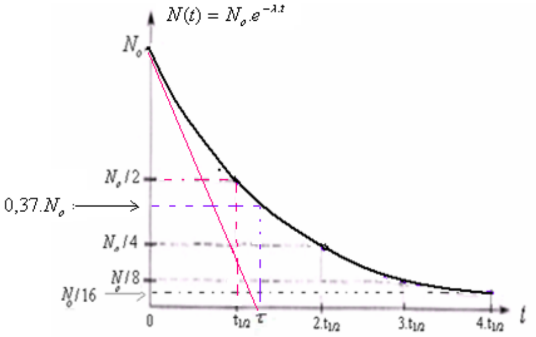
\includegraphics[width=0.5\textwidth]{./img/nuc08.png}
\end{center}

\subsection{Activité d'un échantillon radioactif : }
\section*{Définition : }
On appelle activité d'un échantillon radioactif, le nombre de désintégrations qu'il produits par seconde. $$a(t) = -\frac{dN(t)}{dt}$$
L'activité se mesure en becquerels (Bq) :1Bq correspond à une désintégration par seconde. L'appareil de mesure de l'activité est
appelé: appareil de Geiger.
or $$a(t) = -\frac{N(t)}{dt} = -\frac{N_0.e^{-\lambda.t}}{dt} = \lambda.N(t)$$
d’où: $a(t) = \lambda.N(t)$ et à t=0 on a $a_0 = \lambda.N_0$

donc $$a(t) = a_0.e^{-\lambda.t}$$

En conclusion l'activité est donnée par l'une des relations suivantes: 

$a(t) = \lambda.N(t)$ avec $N(t) = N_0.e^{-\lambda.t}$

$a(t) = a_0.e^{-\lambda.t}$ et $a_0 = \lambda.N_0$

\subsubsection{Datation par radioactivité: }

La radioactivité de certains éléments chimiques qui se trouvent dans les fossiles sédimentaires ou dans les roches permet de déterminer leur âge de la manière suivante:
\begin{itemize}


	\item En mesurant l'activité a(t) de l'échantillon que l'on souhaite dater et l'activité ao d'un échantillon vivant de même nature.
	\item -Et en utilisant la relation : $a(t) = a_0.e^{-\lambda.t}$
		$$ln(\frac{a(t)}{a_0}) = -\lambda.t$$
		donc : $$t = \frac{-\frac{a(t)}{a_0}}{ln(2)} . t_{1/2}$$
\end{itemize}
La datation au carbone 14 est aussi une méthode de datation radioactive basée sur la mesure de l'activité du carbone 14 contenu
dans de la matière organique dont on souhaite connaître l'âge depuis sa mort.

\begin{itemize}

	\item En physique nucléaire le noyau atomique (ou nucléide) est symbolisée par $_Z^AX$ : 
: représente la masse molaire

Ex : pour le nucléide $_{11}^{24}Na$ la masse molaire M(Na) = 24g/mol;

\item 2 ème remarque:
	Or la quantité de matière est donnée par l'une des deux relations suivantes:
	$$n = \frac{m}{M} = \frac{N}{N_a}$$

	donc $$N=\frac{m}{M}.N_a$$

	On peut montrer que $m(t) = m_0.e^{-\lambda.t}$ et $n(t) = n_0.e^{-\lambda.t}$

\item Donc la loi de décroissance radioactive s'applique aussi sur la masse et la quantité de matière radioactive. 





\end{itemize}


\begin{center}

	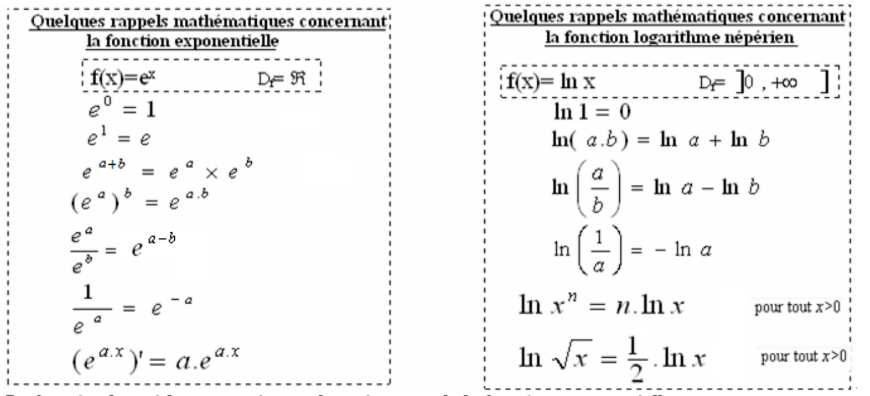
\includegraphics[width=0.5\textwidth]{./img/ex09.png}
\end{center}




%wfg---------------------------------------------------------------sf 
%\begin{center}
   %\begin{tabular}{ |c|c|c|c|c|c|c| }
      %\hline
      %km & hm & dam & \bf{m} & dm & cm & mm \\
      %\hline
        %&   &    &  &   &   & \\
%\hline
%\end{tabular}
%On place un seul nombre dans chaque case.
%\end{center}
%\begin{center}
   %\begin{tabular}{ |c|c|c|c|c|c|c| }
      %\hline
      %$km^2$ & $hm^2$ & $dam^2$ & \bf{$m^2$} & $dm^2$ & $cm^2$ & $mm^2$ \\
      %\hline
        %&   &    &  &   &   & \\
%\hline
%\end{tabular}
%\end{center}


\end{document}

